\documentclass[8pt]{beamer}\usepackage[]{graphicx}\usepackage[]{color}


\usetheme{metropolis}           % Use metropolis theme
\usepackage{amsmath}
\usepackage{mathrsfs}
\usepackage{tabularx}

% For custom oversets
\usepackage{accents}

\def\p#1{\mathbb{P}\left(#1\right)}
\def\q#1{\mathbb{Q}\left(#1\right)}
\def\y{y}
\def\z{z}
\def\normz{\mathcal{N}(z)}
\def\etahat{\hat{\eta}}
\def\ellhat{\hat{\ell}}
\def\sumn{\sum_{n=1}^N}
\def\meann{\frac{1}{N} \sumn}
\newcommand{\etastar}{\accentset{*}{\eta}}
\def\Z{\mathcal{Z}}
\def\expect#1#2{\mathbb{E}_{#1}\left[#2\right]}
\def\kl#1{\mathrm{KL}\left(#1\right)}
\def\klhat#1{\widehat{\mathrm{KL}}\left(#1\right)}
\def\ind#1{1\left(#1\right)}

\DeclareMathOperator*{\argmax}{\mathrm{argmax}}
\DeclareMathOperator*{\argmin}{\mathrm{argmin}}
\DeclareMathOperator*{\esssup}{\mathrm{esssup}}
\DeclareMathOperator*{\essinf}{\mathrm{essinf}}
\DeclareMathOperator*{\argsup}{\mathrm{argsup}}
\DeclareMathOperator*{\arginf}{\mathrm{arginf}}

\title{Deterministic Automatic Differentiation Variational Inference}
\author{Ryan Giordano}
\date{Sep 23rd, 2022}
\institute{Massachusetts Institute of Technology}

\begin{document}




%%%%%%%%%%%%%%%%%%%%%%%%%%%%%%%%%%%%%%%%%%%%%%%%%%%%%%%%%%%%%%%%%%%%%%%
%%%%%%%%%%%%%%%%%%%%%%%%%%%%%%%%%%%%%%%%%%%%%%%%%%%%%%%%%%%%%%%%%%%%%%%
%%%%%%%%%%%%%%%%%%%%%%%%%%%%%%%%%%%%%%%%%%%%%%%%%%%%%%%%%%%%%%%%%%%%%%%

\begin{frame}{Black box variational Inference}
%
``Black box variational Inference'' (BBVI) is a set of techniques for quickly and
{\em automatically} approximating Bayesian posteriors using optimization. I'll
consider ``mean field automatic differentiation variational inference'' (ADVI).

\pause
Let $\theta$ denote model parameters and $\y$ some data and the joint
generating distribution be $\p{\theta, \y} = \p{\y \vert \theta} \p{\theta}$.
Let $\q{\theta \vert \eta}$ be a family of candidate approximate posteriors,
here taken to be independent normals.

ADVI aims to find
%
\begin{align*}
%
\etastar :=
    \argmin_{\eta} \kl{\q{\theta \vert \eta} || \p{\theta \vert \y}}
    = \argmin_{\eta} \expect{\normz}{f(\z  | \eta)}
%
\end{align*}
%
for a cleverly constructed, automatically-differentiable $\eta \mapsto f(\z |
\eta)$.

\pause
Unfortunately, $\expect{\normz}{f(\z  | \eta)}$ is typically intractable. So
ADVI uses stochastic gradient (SG).  The leads to the following problems:
%
\begin{itemize}
%
\item You have to tune the step size carefully
\item You can't assess convergence directly
\item You can't compute sensitivity, so you can't use linear response
covariances.
%
\end{itemize}
%
$\Rightarrow$ Optimization is slow and imprecise, and the posterior uncertainty
is no good.  Not so black box actually!

\textbf{
We propose a simple alternative to SG that resolves these
problems (sometimes).
}

%
\end{frame}



%%%%%%%%%%%%%%%%%%%%%%%%%%%%%%%%%%%%%%%%%%%%%%%%%%%%%%%%%%%%%%%%%%%%%%%
%%%%%%%%%%%%%%%%%%%%%%%%%%%%%%%%%%%%%%%%%%%%%%%%%%%%%%%%%%%%%%%%%%%%%%%
%%%%%%%%%%%%%%%%%%%%%%%%%%%%%%%%%%%%%%%%%%%%%%%%%%%%%%%%%%%%%%%%%%%%%%%

\begin{frame}{Optimization of intractable expectations}
%
Suppse you want to minimize an objective function of the form
%
\begin{align*}
%
\etastar :=  \argmin_{\eta} \expect{\p{\z}}{f(\z | \eta)}
:= \argmin_{\eta} \ell(\eta),
%
\end{align*}
%
where $\p{\z}$ is known, but the expectation is not available in closed form.

\pause
When does this happen?
%
\begin{itemize}
%
\item Black box variational inference
%
\item Stochastic control (e.g. you have a factory, and supply and demand are
random)
%
\end{itemize}
%
\pause What can you do?  There are two options, both using the Monte Carlo (MC)
estimate
%
\begin{align*}
%
\ellhat(\eta) := \meann f(z_n | \eta) \approx \ell(\eta).
%
\end{align*}
%
\pause
%
\begin{itemize}
%
\item Stochastic gradient (SG)
%
\begin{itemize}
%
\item Update with $\eta^{i} = \eta^{i-1} - \rho \nabla_\eta \ellhat(\eta)$
for some step size $\rho$ (new $\z_n$ every step)
\item Approximately minimizes the exact objective
%
\end{itemize}
%
\pause
\item Sample average approximation (SAA)
%
\begin{itemize}
%
\item Find $\etahat := \argmin_{\eta} \ellhat(\eta)$ for fixed $\z_n$
\item Exactly minimizes approximate objective
%
\end{itemize}
%
\end{itemize}
%
\pause
Which is better? \textbf{In general, it depends.}


As far as we can tell, the BBVI literature has only ever considered SG.
%
\end{frame}




%%%%%%%%%%%%%%%%%%%%%%%%%%%%%%%%%%%%%%%%%%%%%%%%%%%%%%%%%%%%%%%%%%%%%%%
%%%%%%%%%%%%%%%%%%%%%%%%%%%%%%%%%%%%%%%%%%%%%%%%%%%%%%%%%%%%%%%%%%%%%%%
%%%%%%%%%%%%%%%%%%%%%%%%%%%%%%%%%%%%%%%%%%%%%%%%%%%%%%%%%%%%%%%%%%%%%%%

\begin{frame}{Optimization of intractable expectations}

\begin{minipage}[t]{0.45\linewidth}
    %
    Sample average approximation (SAA)
    %
    \begin{itemize}
    %
    \item Find $\etahat := \argmin_{\eta} \ellhat(\eta)$
    \item Fixed $\z_n$ for whole procedure
    \item Exactly minimizes approximate objective
    %
    \end{itemize}

\onslide<2->{
\textbf{Advantages:}
%
\begin{itemize}
%
\item Can use fast off-the-shelf second-order optimization (great for
poorly-conditioned problems)
\item Can evaluate the objective function exactly to check for convergence
\item Can compute sensitivity (linear response covariances $\Rightarrow$
more accurate posterior covariances for mean field approximations)
%
\end{itemize}
}
%
\end{minipage}
\hfill\vline\hfill
\begin{minipage}[t]{0.45\linewidth}
    %
    Stochastic gradient (SG)
    %
    \begin{itemize}
    %
    \item $\eta^{i} = \eta^{i-1} - \rho \nabla_\eta \ellhat(\eta)$
    \item New $\z_n$ every step
    \item Approximately minimizes the exact objective
    %
    \end{itemize}

\onslide<3->{
\textbf{Advantages:}
%
\begin{itemize}
%
\item Uses each draw $\z_n$ only once (for a single gradient step)
%
\end{itemize}
}
%
\onslide<4->{
This is actually a big one!  Because if $\eta \in \mathbb{R}^D$,
in general, both
SG and SAA have accuracy $(D / N)^{-1/2}$, where $N$ is the {\em total}
number of draws of $\z_n$ used.

\vspace{1em}
SAA uses each draw at each step of optimization.  SG uses each draw once.
%
%\vspace{1em}

$\Rightarrow$ In general, SG is much more efficient in high dimensions!
}
%
\end{minipage}

\hrulefill

\onslide<5->{
\textbf{Theorem (us).}  If $\log \p{\theta, \y}$ is high dimensional
due to a large number of ``local'' variables, then the accuracy
is $~ (\log D / N)^{-1/2}$, rendering SAA feasible.
}
\end{frame}

\begin{frame}{Experimental results: Runtime}
    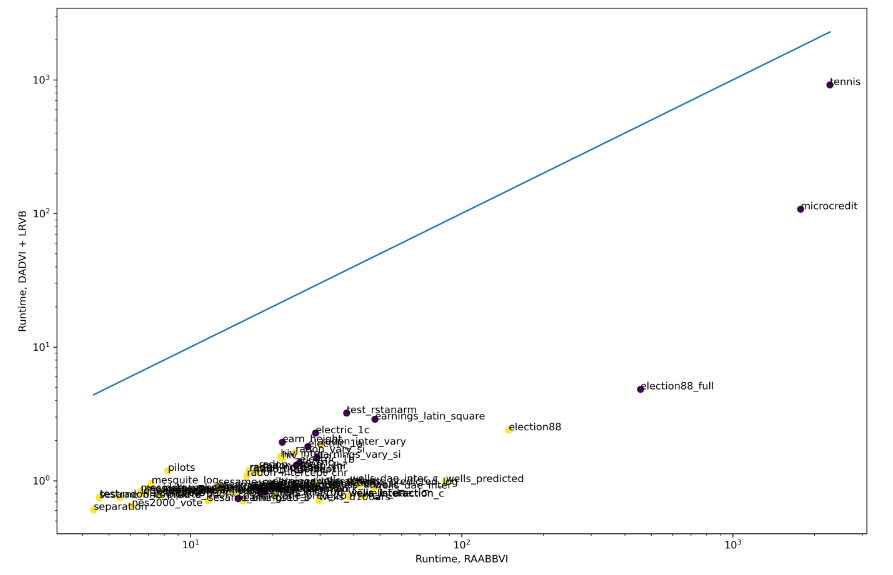
\includegraphics[width=0.9\linewidth]{runtime}
\end{frame}

\begin{frame}{Experimental results: Means}
    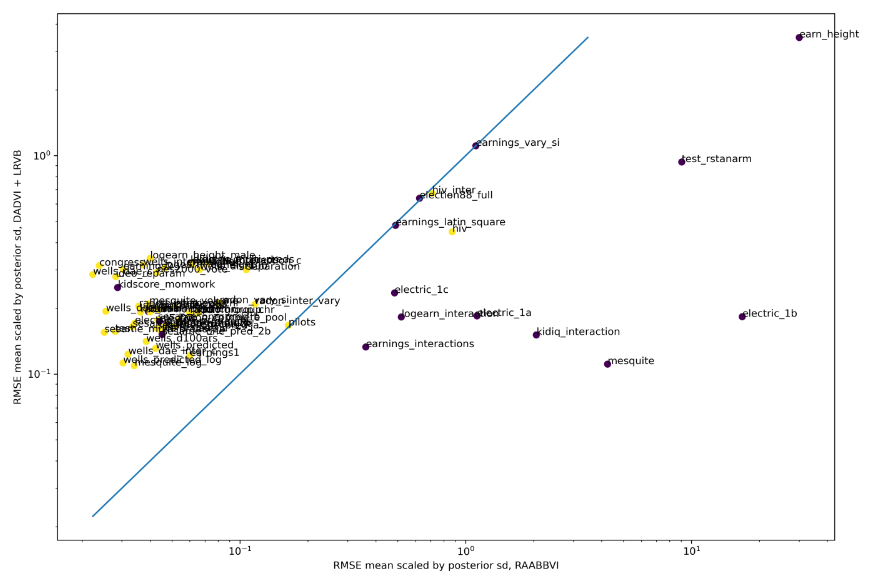
\includegraphics[width=0.9\linewidth]{means}
\end{frame}

\begin{frame}{Experimental results: Standard deviations}
    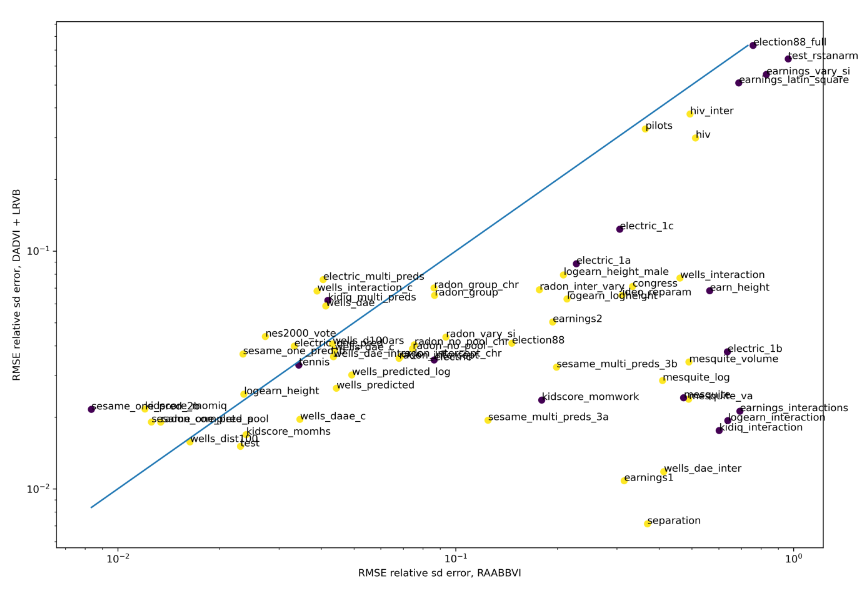
\includegraphics[width=0.9\linewidth]{sd}
\end{frame}

\end{document}
